\documentclass [8 pt]{article}
\usepackage[utf8]{inputenc}
\usepackage[T1]{fontenc}
\usepackage{geometry}
\usepackage{graphicx}
\graphicspath{{images/}}
\geometry{a4paper}
\usepackage{helvet}
\newcommand\tab[1][1cm]{\hspace*{#1}}
\renewcommand{\familydefault}{\sfdefault}
\begin {document}
\begin {titlepage}
\vspace *{\fill}
\begin {center}
\Huge{\textbf{EXAMINATION MALPRACTICE IN MAKERERE UNIVERSITY}}\\ [2CM]
\Large { AMPAIRE WILFUL 15/U/21173 }  

  $20^{th} May 2017$\\ 
\setlength{\topmargin}{-1cm}
\end {center}
\vspace *{\fill}
\end {titlepage}


\large {\textbf {ABSTRACT}}\\
The study investigated perception of students on factors accountable for examination malpractices in Makerere University. The study is a qualitative or descriptive study where some students were chosen randomly to provide there ideals about why students cheat examinations, the methods they use, and what could be the possible solutions. 
\section {INTRODUCTION}
Examination malpractices has been a common habit among students of Makerere for a while which contravenes the rules and regulations set by examination bodies and  which gives a bad image to university especially in other universities that look at Makerere as the biggest university in Africa. So data collection has been made using qualitative research and it was found out that the major cause is indiscipline among students by not preparing for the examinations in time. According to research, examination malpractice can be reduced by suspending or expelling of students that involve in this habit, and carrying out effective supervision of students during examinations
\subsection { Background}
Examination malpractice has almost be a habit among students of Makarere and some students still do it which spoils name of the university and some student that participate it end up not getting their transcripts at the end of their academics . Supervision of examinations have been somewhat improved but still the problem is persisting. Therefore we can resort to other ways of solving this problem like using CCTV cameras, doing online exams and so on.
\subsection {Objective}
To discover the approaches students use to cheat the examination system.
To discover the reasons why students get involved in examination malpractice.
To discover possible ways through which ICTs can be used to stop the problem.
\section { METHODOLOGY}
\subsection {Research questions}
 The following were the guiding questions which helped me in collecting data around the problem domain;
\begin {enumerate}
\item  Why do you think students get involved in examination malpractices in Makerere University?
\item What kind of methods do you think the students use to cheat examinations?
\item What possible ways through which ICT solutions can be used to stop the problem?

\end{enumerate}
\subsection {Measurement instruments}
Data was collected using the forms that were created using the ODK build and then transferred to an android phone. After filling the forms they are sent to the ODK aggregate server 

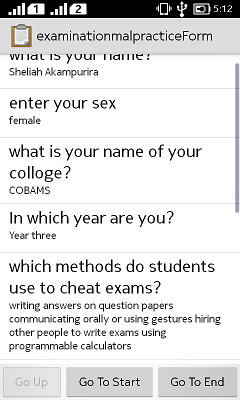
\includegraphics{pic1}


\subsection {Data analysis}
According to the collected information and data, the leading factors as to why students involve in examination malpractice is the desire to pass exams at all cost which is due to lack of confidence and fear of getting low marks as well as being ill prepared for the examination. Other reasons are the anxiety to get a certificate and high-grade and the emphasis on certificate presentation for a job, Improper guidance and counseling, truancy, absenteeism and laziness attribute to this ill-preparedness for examinations. 
\newline While some students intentionally get indulge in the malpractices; others see themselves in it through ignorance, carelessness or forgetfulness in applying regulations or due to peer pressure. The methods that are often used include writing answers on question papers, copying other students work during the examination entering examination room with phones, lecturers sending prepared answers to students writing on body parts hiring other people to write exams, using programmable calculators. 

The table below summarises the respondents view on devices and methods used in examination malpractices in Makerere University 

\begin{center}
\begin{tabular}{||c |c |c |c||}
\hline Responses & Agree & Disagree & Maybe\\
[0.5ex]
\hline
\hline  hiring  other people to write examinations  & 60  & 25 & 15 \\
\hline sending prepared answers to students  & 80 & 20& 0\\
\hline copying copying other students' work during examination & 65  & 20 & 15 \\
\hline entering examination rooms with prepared answers & 85 & 5 & 10 \\
\hline leakage of examinations before sitting for it & 50 & 50 & 0  \\
\hline writing on body parts & 85  & 10 & 5 \\
\hline communicating orally or using gestures & 83  & 10 & 7 \\
\hline writing answers on question papers & 90 & 10 &  0 \\
\hline using programmable calculators during examination& 70 & 25 & 5\\
\hline hiding materials in washrooms, pockets and private parts & 90 & 10 & 0  \\
[0.5ex]
\hline 
\end{tabular}
\end{center}
	 

\subsection {Research sample }
The study will include both males and females of different age groups and which will be grouped in focus group discussions of students each in a group and the random sampling method will be used to carry out a sample of the findings. 
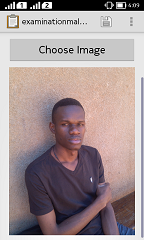
\includegraphics{pic5}
\includegraphics{pic6}
\section {Discussion}
The foregoing shows the analysis of data collected for this study.as indicated in the findings one of the reasons why students get involved in examination malpractice is due lack of strengthening and implementing seriously the penalties so students take it to be light when doing it since the culprits are usually forgiven to some extent and lack of installation of ICT systems in the examination rooms and the whole corners of the buildings in makerere university in different colleges.

\section {Conclusion}
Considering the findings of the study, it was concluded that indiscipline among students by not preparing in time for examinations is critical variable in students’ involvement in examination in examination malpractices in the university. This was evident in the findings which singled out lack of enough preparation for examinations as a root reason why students get involved in the examination malpractice. The findings have also led to the conclusion that effective supervision of students during examinations is lacking in the university.
\section {Recommendations}
Grounded on the findings of this study, students recommended that there should be installation of ICT systems for example CCTV cameras in examination rooms to ease the supervision and eradicate examination malpractice in Makerere University. There was a conclusion on doing examination online and the system marks and award marks to students immediately so that a student goes knowing his/her marks scored and this will reduce and eradicate examination malpractice in makerere university.
Concerted efforts should be made in enhancing discipline among students through the counselling services in the university to prevent them from the act of indiscipline during examinations. Electronic devices should be used to check students’ pockets before entering examination rooms.
There should be increased efforts by principals in the university and examination boards in enhancing the effective supervision of students during examination.


\end{document}



